\label{chap:framework}
This chapter discusses the Self-Aware FramEwork (SAFE) developed to test and experiment with self-aware and self-adaptive control policies. SAFE is a simulation framework designed to execute instruction traces broken into energies per operation. SAFE simulates a 2048 core exascale architecture integrated circuit organized into a three level hierarchy. The simulated chip consist of 16 units organized into 16 blocks; where each block consist of 8 execution engines and a single control engine. Additionally, SAFE incorporates thermal simulation modeling of heat distribution among blocks of the chip. In order to facilitate adaptation and to more accurately model chip communication, SAFE incorporates a tiered approach to communication of messages between blocks within the chip. Figure \ref{fig:AMM} shows our Target Exascale Architecture (TEA) mapped to control engines. Though we only simulate a single chip, we envision the control hierarchy of SAFE to extend across chips in an exascale system.

\begin{figure}[htb!]
    \centering
    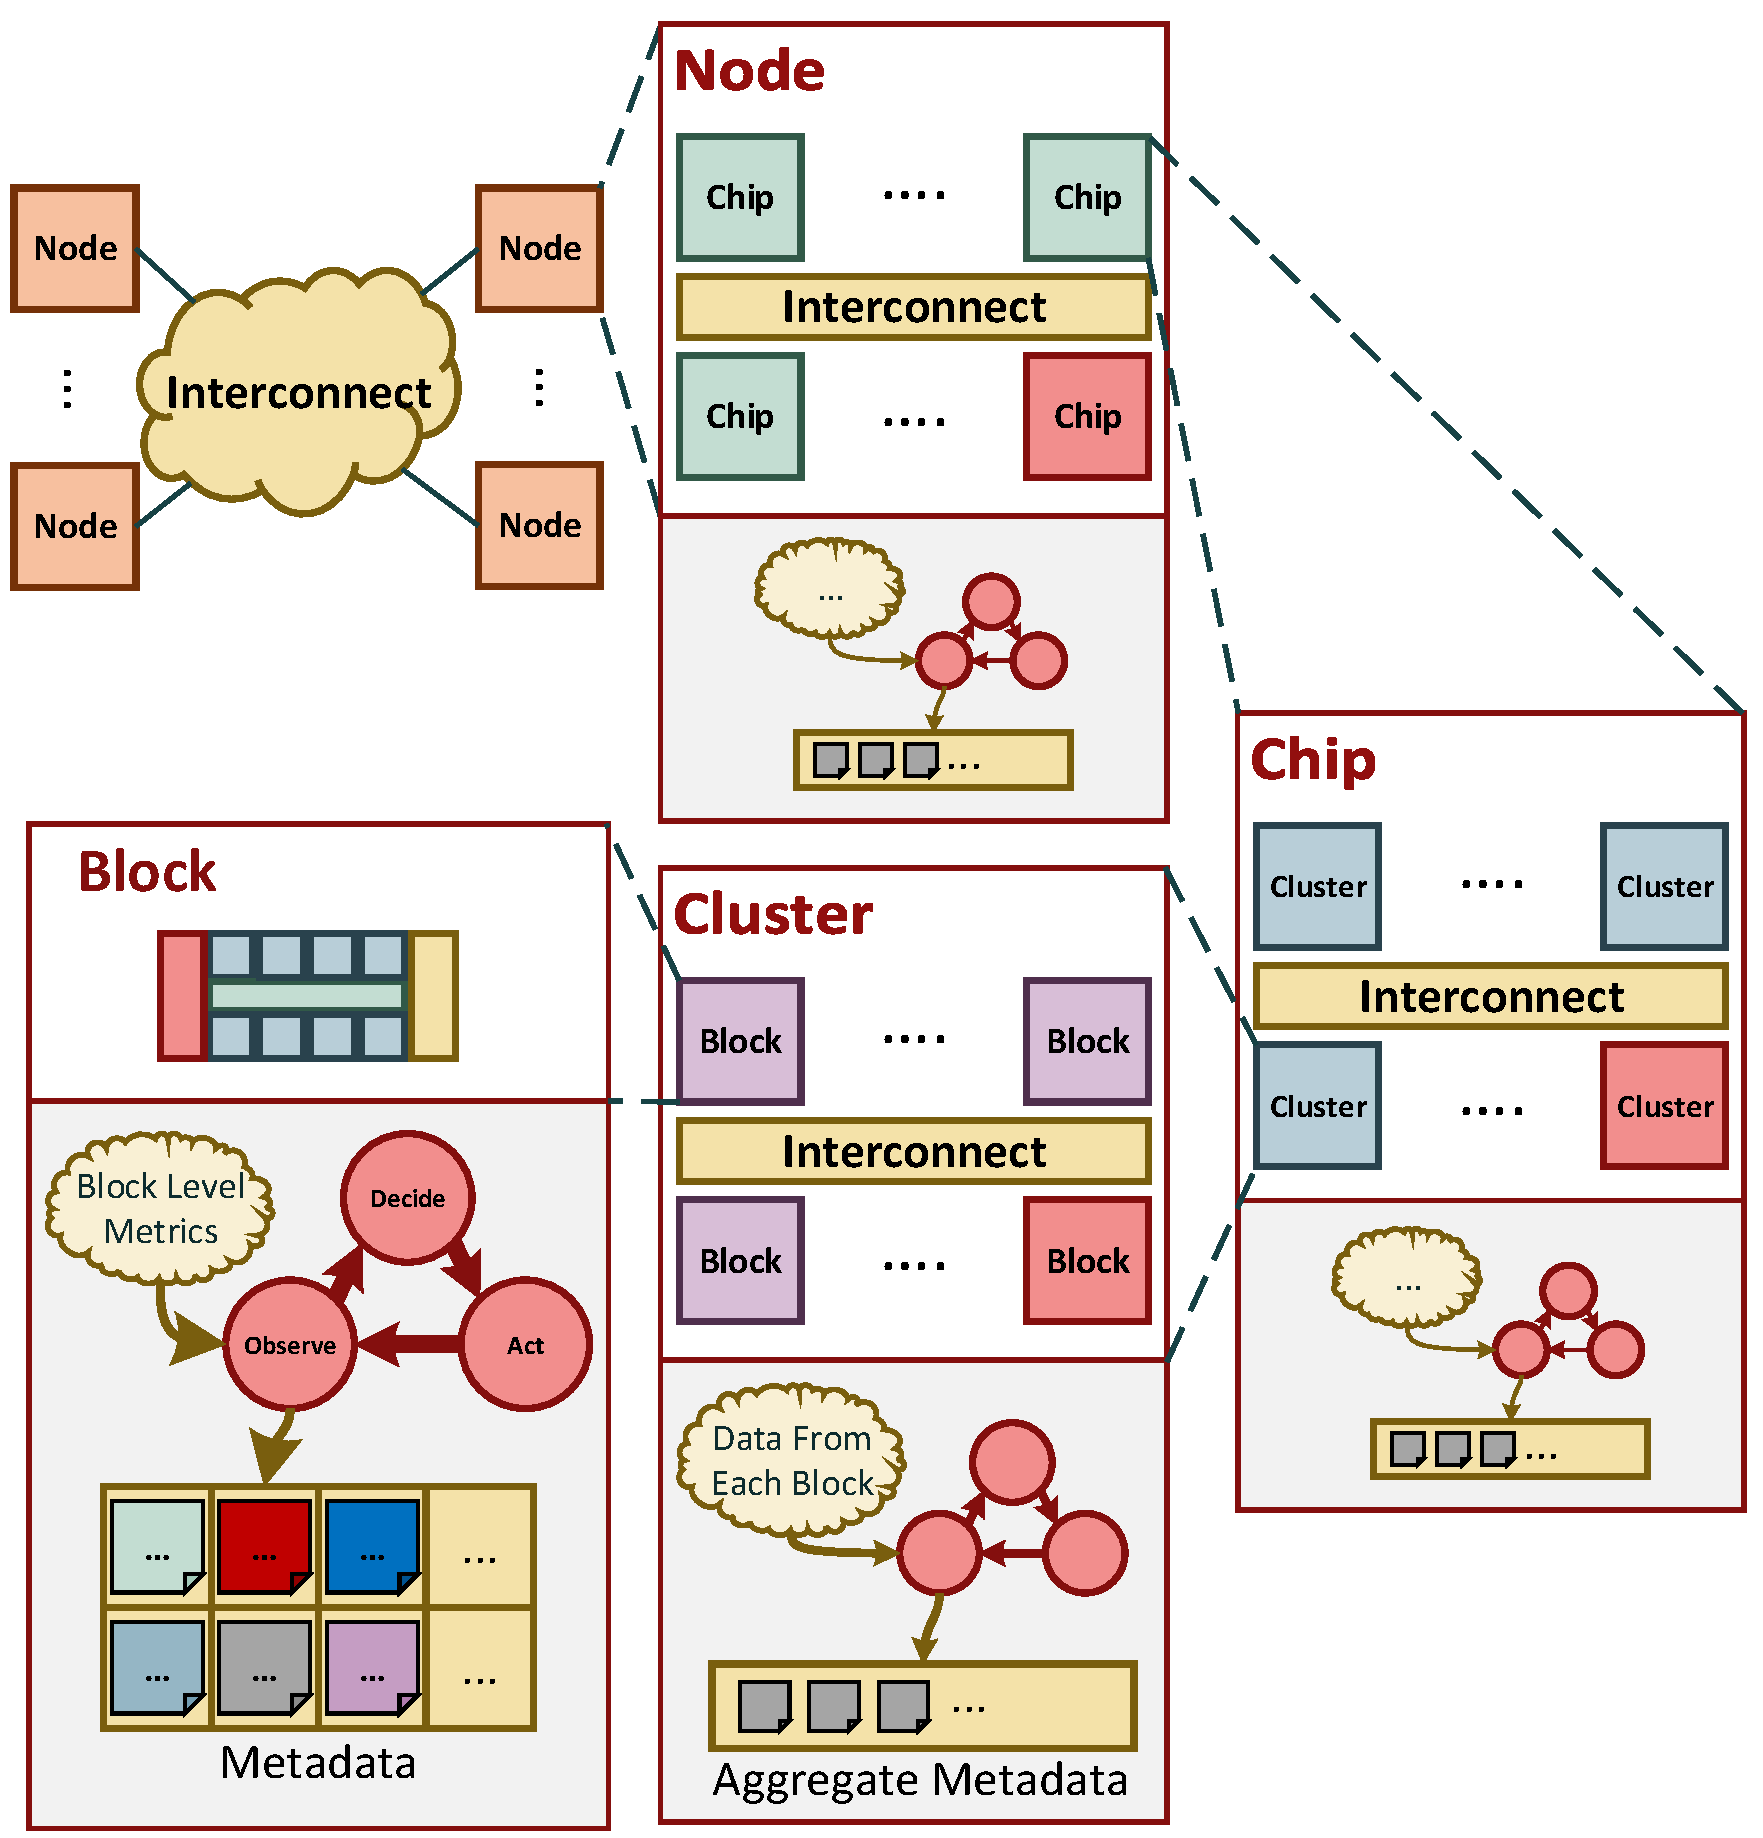
\includegraphics[width=0.95\textwidth]{Fig/AMM.pdf}
    \caption[Abstract Machine Model with Adaption]{Abstract Machine Model with Adaption: Shown is an abstract representation of the TEA with control engines operating at each level of the hierarchy.}
    \label{fig:AMM}
\end{figure} 

The following sections discuss SAFE in more detail. First, we discuss the various models built into SAFE and then move into a discussion of adaptive policy implementation.

\section{Execution and Energy Modeling}
%{
    SAFE models the execution of individual instructions in terms of their energy expended during operation. Instructions are grouped into two types: low energy operations with full and near threshold voltage (NTV) state energies, and memory operations that use high amounts of energy where energy doesn't change regardless of the DVFS state of components within the block. Energy is accumulated on a per block basis and this is used to compute temperatures as discussed in section~\ref{thermal_model}. A simple power window taking into account a configurable amount of cycles is used in conjunction with chip clock rates to compute the current power of a block.

    All blocks within SAFE operate independently and periodically synchronize to reduce skew in execution results. Each block is capable of adjusting the execution state of individual execution engines within it between full frequency and NTV in order to facilitate adaptation. Additionally, block control engines have control over network access of memory requests moving in and out of the block and can choose to throttle network activity in terms of percentages. This is a requirement because heavy network traffic will necessarily result in high energy expenditure.

    SAFE also incorporates an instruction consolidation mechanism in order to reduce simulation run times. Essentially, it uses the law of averages to merge multiple instructions into a single instruction and reduce the real time execution of a given simulation. This is configurable on a per run basis. Finally, SAFE models DRAM port access in order to more realistically limit network energy. This is configurable on a per port basis at an individual block level.
%}

\section{Control Engine Modeling}
%{
    \label{ControlEngineModeling}
    SAFE incorporates a 3 level tiered distributed control hierarchy among blocks. At the top level, a chip control engine dictates power and temperature goals to units under its control. Unit control engines further dictate power and temperature goals to blocks under their control based on the goal dictated from the chip. At the lowest level, block control engines directly control execution engine DVFS states by individually throttling cores between full frequency and near threshold voltage (NTV). As discussed in the prior section, Full and NTV states consist of differing amount of joules. In essence, SAFE models a distributed and hierarchical system between control engines at different levels. Figure~\ref{fig:Control-Hierarchy} illustrates the control hierarchy. 

    \begin{figure}[htb!]
        \centering
        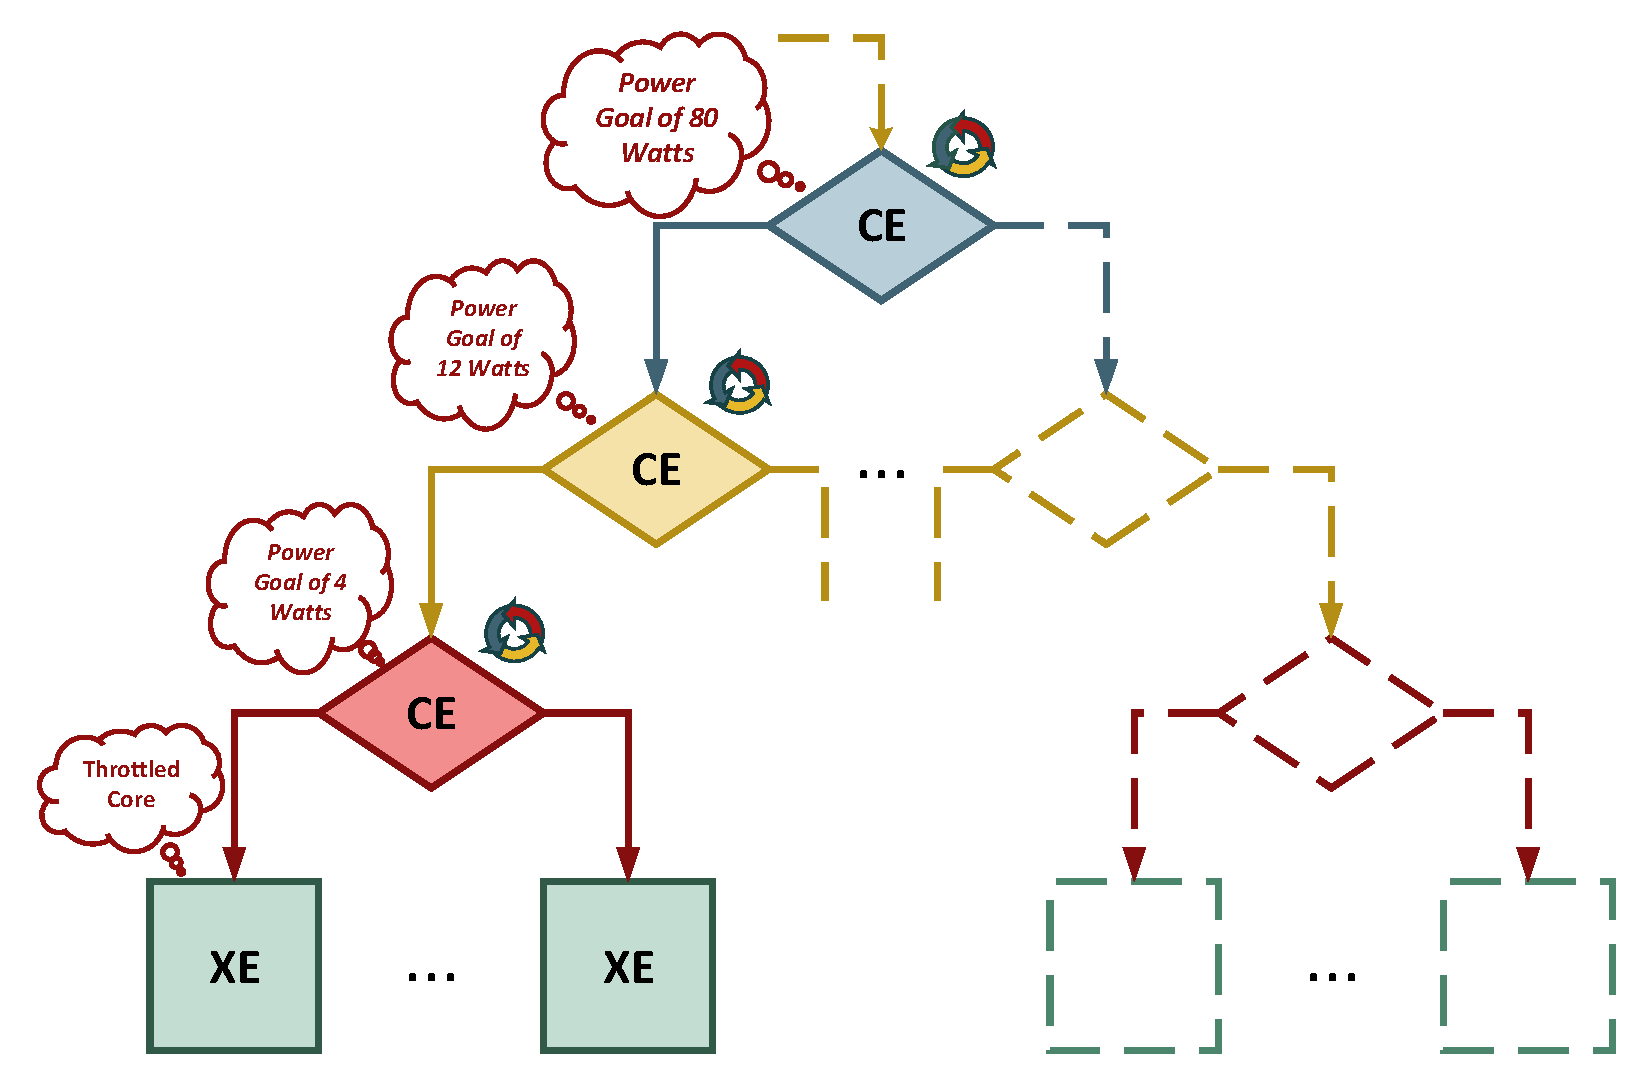
\includegraphics[width=1.0\textwidth]{Fig/Control_Hierarchy.pdf}
        \caption[SAFE Control Hierarchy]{SAFE Control Hierarchy: A generalized example of SAFE's control hierarchy. On the left decisions are shown moving down the hierarchy. The circular arrows indicate that observe-decide-act mechanisms are occurring within each CE. As shown, goals are relative to the central goal dictated by the root CE.}
        \label{fig:Control-Hierarchy}
    \end{figure}

    Additionally, block control engines throttle network activity under their own discretion on a per block basis. Network throttling simulates bandwidth tapering by reducing the network communication from full speed to some percentage of the full speed. This necessarily causes increased latency for memory operations but reduces energy consumption and thus power. Network throttling is necessary for adaptive power and thermal control of bandwidth intensive applications without which, power and temperature goals will unable to be met.

    Control engines dictate adaptive goals to components under their control indirectly or directly. These said goals are decided through observation of system state either indirectly or directly. For example, direct observation would entail a temperature machine specific register (MSR), and indirect observation would entail the aggregation of temperatures among higher level control engines in the hierarchy. These observations are used in an observe-decide-act (ODA) loop to either make decisions about goals (at higher level tiered control engines) or to directly tweak control knobs (e.g. adjust DVFS state, etc.). In essence, the system entails a distributed control hierarchy synergistically making decisions to meet the highest level goal dictated by the chip level control engine. This goal is propagated down and lower level control engines decide how to allocate their own goals toward meeting this overall goal. 
%}

\section{Data Aggregation}
%{
    SAFE aggregates directly observed data to parent control engines and pushes it up the control hierarchy. That is to say, data is distilled and aggregated up the hierarchy for control engines to make decisions upon. This is further distilled as it moves up the hierarchy. This relationship is shown in figure~\ref{fig:Data-Hierarchy}. The aggregated data is statistical information detailing the state of the components under control of a given control engine. SAFE employs probability theory in terms of central moments to meaningfully characterize data distributions across the simulated system. Currently, the implemented control policies only use the first moment (average) for decision making, but more complex policies could incorporate variance and skewness; as well as, implement other types of data to be aggregated (such as memory movement information). Variance and skewness give a notion about the spread of a distribution, as well as, any asymmetry presence respectively. The rest of this section is devoted to discussing the use case of the various moments for purposes of adaptation. 


     \begin{figure}[htb!]
        \centering
        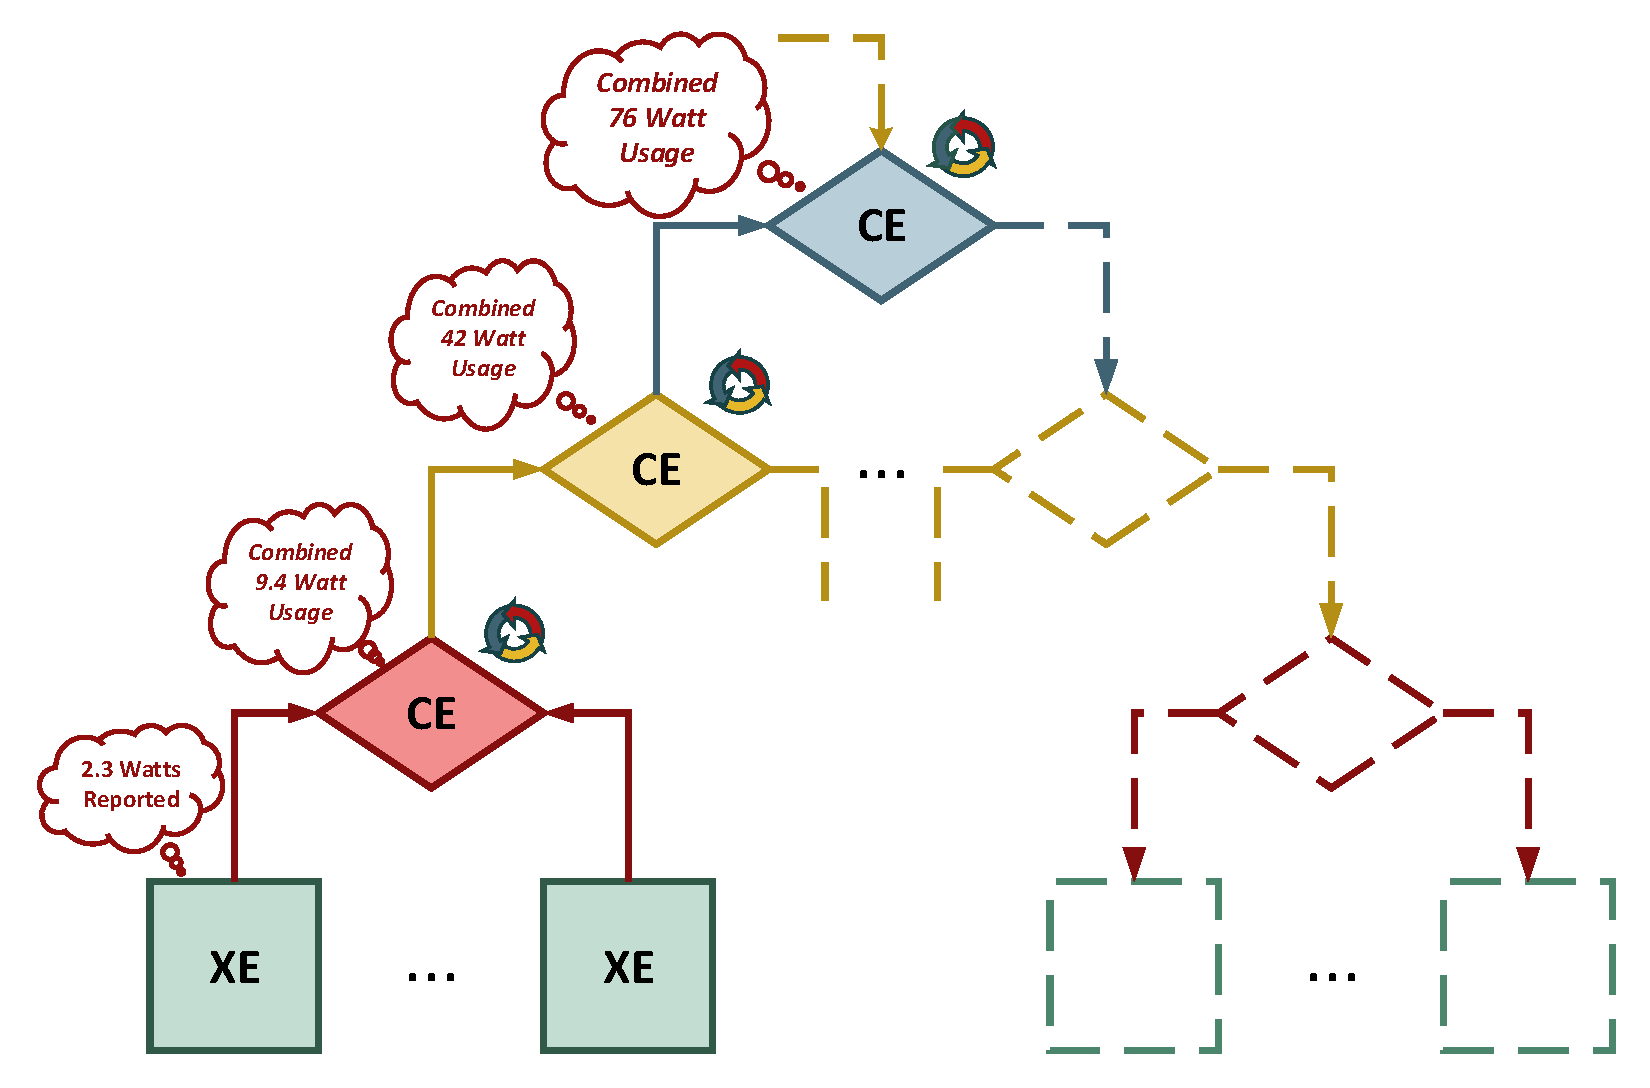
\includegraphics[width=1.0\textwidth]{Fig/Data_Hierarchy.pdf}
        \caption[SAFE Aggregated Data Hierarchy]{SAFE Aggregated Data Hierarchy: A generalized example of SAFE's data aggregation hierarchy. The left shows data aggregation moving up the hierarchy. The circular arrows indicate observe-decide-act mechanisms are occurring within each CE. As shown, the combined wattage is aggregated at the top of the hierarchy for the root CE to make decision upon and dictate subgoals to lower level control engines. These subgoals are further divided as the control engines propagate them down the hierarchy. The individual allocations at each level are completely up to the parent control engine at each level.}
        \label{fig:Data-Hierarchy}
    \end{figure}
    
    In detailed terms, variance can provide a control engine with a notion of system imbalance. Within an exascale architecture, imbalance may be the result of process and circuit variance, run-time induced variance, and inherent-program variance. Skewness on the other hand, can provide a notion of hot spotting within a system that be the result of the previously mentioned sources. Variance and skew could be used in conjunction with an intelligent scheduler for adaptive scheduling.

    Finally, it is worth noting that the task of aggregation is burdened by two important design constraints: (1) the need to characterize temperature and power distributions accurately, and (2) the need to minimize communication and performance costs across the system. These two design goals can be seen as conflicting in nature in that minimizing communication and performance costs necessarily decreases the amount and accuracy of information one can move around the system. One design goal of SAFE was in minimizing communication while maintaining accurate and up-to-date information across the hierarchy. The communication model used within SAFE is discussed in the following section.

%}

\section{Communication Modeling}
%{
    SAFE incorporates a simple communication protocol consisting of mailboxes for communicating between control engines. Each control engine has reserved slots for receiving control information from its parent and aggregated data from its children. Messages are designed to minimize data-transfer while maintaining data integrity in terms of accuracy. A control engine is responsible for checking the slot and emptying its contents for more data to be placed within. A simple queuing system is used in the case that messages become backlogged for any reason (i.e. the control engine doesn't service them fast enough). In order, to minimize stale data, any queued messages are checked and old messages of the same type are replaced. This has the effect of aiding response time during the decision making process.

    The communication protocol consists of 64-bit messages in order to minimize data transfer. Minimizing data transfer is central to the design of SAFE's communication hierarchy as large transfers would necessarily result in high energy costs which contradicts the goal of SAFE to manage power and temperature, as mentioned the prior section. Additionally, minimizing data transfers also speeds up communication to allow for better adaptation. In terms of hardware, such a communication network might use specialized hardware tailored to message size and type to further improve efficiency.

    Messages in SAFE are broken up into a 4-bit header, and 28 reserved bits depending on message type. Temperature data is encoded as 8-bits and power is encoded as 16-bits. The encoding scheme for temperature uses a simple 2-bit fractional encoding for fractional temperatures, reserving the upper 6 bits for the whole number portion. Figure~\ref{fig:Example-Encoding} shows the fractional bit encoding scheme for temperature. Essentially, values are encoded in terms of notches always rounding up. For example, a temperature of 76.1 degrees Celsius would be encoded as 76.25 degrees Celsius using the encoding. The whole number encoding size was chosen based off of how modern architectures encode temperature. These typically provide 12 to 13 bit precision MSRs encoding a temperature differential which is then subtracted from a thermal junction design point to calculate the actual temperature. For example, some processors use 127 degrees Celsius and others 100 degrees Celsius as the thermal junction design point. SAFE implements the same mechanism using 100 degrees Celsius as the thermal design point. However because ambient temperature is 50 degrees Celsius and maximum operating temperature is 100 degrees Celsius, only 6-bits are needed to represent all possible values.


     \begin{figure}[htb!]
        \centering
        \begin{tcolorbox}[tabularx={X|X},title=Fraction Bit Encoding for Temperature,boxrule=0.25pt]
         Bit Encoding & Fractional Interpretation \\ \hline
         0b00 & 0.00 \\ \hline
         0b01 & 0.25 \\ \hline
         0b10 & 0.50 \\ \hline
         0b11 & 0.75 \\ \hline
         0bXX & ...  \\ \hline
        \end{tcolorbox}
        \caption[Fraction Bit Encoding for Temperature]{The left column shows an example bit encoding of temperature. The right column shows an example notch pairing.}
        \label{fig:Example-Encoding}
    \end{figure}

    Power is more complicated to encode because it ranges from fractional values at the lowest level to large values at the highest levels when aggregated. Accurately representing this can be a challenge when attempting to preserve precision and accuracy. The employed encoding scheme takes a maximum possible encodable value (e.g. 30 watts) and then uses this value to determine individual evenly spread representable notch values. For example, an encoding scheme might have notches of 0.04, 0.08, 0.012, so on so forth. The actual values of the notches depend on the bit-width size employed. A 16-bit encoding size was decided by testing the accuracy of adaptive policies at various precisions. This allows for 65536 possible values to be encoded. Given a 30 watt maximum, this would allow for individual notches of 457.76 microjoules to be encoded. Employing a different maximum encodable value at differing levels of the control hierarchy allows for varying precisions that fit aggregated value ranges on a per level basis.

%}

\section{Thermal Modeling}
%{
    \label{thermal_model}
    SAFE incorporates a linear heat simulation of localized heat and temperature using thermal conductivity and thermal resistivity based off of a prior model~\cite{Livingston2015}. In the model, localized heat dissipates across the chip over time. SAFE models a 500 by 500 millimeter chip with a heat sink installed across the top. Figure~\ref{fig:Heat-Distribution} shows a possible heat distribution in a 3 by 3 grid of blocks.

     \begin{figure}[htb!]
        \centering
        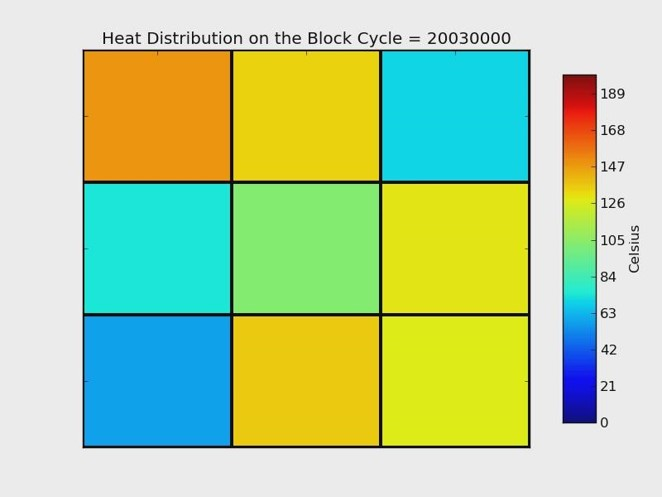
\includegraphics[width=0.6\textwidth]{Fig/temp_distribution.jpg}
        \caption[Example Heat Distribution in a 3 by 3 Grid of Blocks]{Example Heat Distribution in a 3 by 3 Grid of Blocks: Due to number of cores and small area of blocks on the simulated chip, high differentials in temperatures are possible and localized heat could lead to hot spotting.}
        \label{fig:Heat-Distribution}
    \end{figure}

    Heat is modeled in terms of joules accumulated on a per block basis for a 256 block simulation. The model incorporates a tiled layout where each interior block has 4 neighbors (top, bottom, left, right). Exterior blocks have 3 or 2 neighbors depending on whether they are located on an edge or corner respectively. Heat is dissipated across neighbor blocks asynchronously as it accumulates, as well as, to the heat sink located along the top which is modeled at a configurable ambient temperature. Figure~\ref{fig:CrossSection} shows a cross sectional view of a block and its neighbors. The amount of heat flux moving in or out of a block depends on the temperature gradient between the respective components. This is modeled as a simple linearly transfer because the chip does not operate at temperatures where one would see a non-linear relationship. For example, a block operating at 70 degrees Celsius will transfer heat to the heat sink at a linearly lower rate than another operating at 80 degrees Celsius.

     \begin{figure}[htb!]
        \centering
        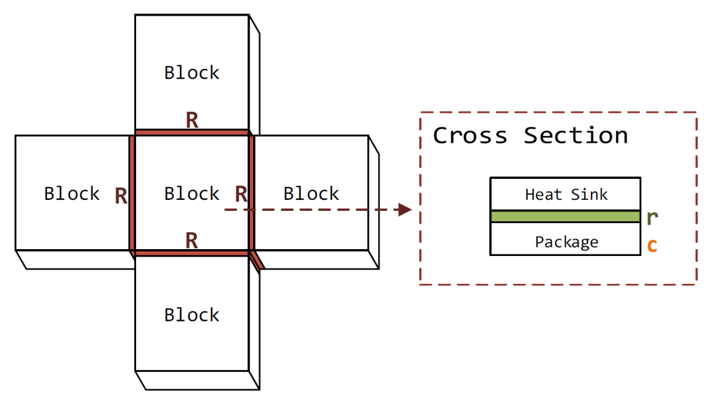
\includegraphics[width=0.8\textwidth]{Fig/Block-CrossSection.png}
        \caption[Cross-sectional View of an Individual Block and Neighbors]{Cross-sectional View of an Individual Block and Neighbors: Heat radiates along the four boundaries between neighbors and across the heat sink along the top.}
        \label{fig:CrossSection}
    \end{figure}

    Specifically, in terms of modeling, heat is translated into temperature (in degrees Celsius) based on the specific heat and density of silicon, the wafer density, and the size of the chip. For heat dissipation across the heat sink, thermal conductivity, and the size of the chip is used. The thermal conductivity has been calibrated such that an average 100 watt workload across the chip will stabilize the temperature to 100 degrees Celsius. Heat dissipation to neighbors is modeled using a conductivity constant, the physical distance between blocks in terms of micrometers, as well as the block width and height. All of the parameters are configurable for use with a generalized chip outside of the one modeled in this thesis.

    A key aspect of the temperature model, is that temperature can be used to implement adaptive policies to meet average temperature goals across the chip. Additionally, adaptive wattage goals can be used to indirectly meet temperature goals. This is discussed in more detail within Chapter~\ref{chap:results}. Though, not explored within this thesis, temperature variance, as well as skew could be used to further refine adaptive policies. 
%}


\section{Control Policies}
%{
    SAFE is a framework designed to implement and test various control policies for adaptation, as well as, to explore the types of data needed to enable adaptive policies. Each of the tiered control engines discussed in section~\ref{ControlEngineModeling} implement separate control policies for their respective sections of the system. How a policy is implemented naturally depends on the level in the hierarchy.

    At the lowest level control engines have direct control over components at their disposal. They can throttle networking activity or individually adjust the DVFS states of blocks. Additionally, they can read MSRs to collect information about their state. Currently, temperature, power, and network activity MSRs are implemented and used in implemented adaptive policies. Higher level control engines have indirect control over hardware. They receive aggregated statistics from lower level control engines and use this information to make informed policy decisions. In terms of control, they give goals in terms of power or temperature to lower level control engines. The design of SAFE allows for more complicated control messages to be easily implemented. The details of the implemented policies are discussed in Section \ref{sec:policies}.
%}








